\section{Operational Concept Description}


\subsection{Shared Vision}

	\subsubsection{System Overview}\begin{multicols}{2}
				\paragraph{Key Partners}\begin{enumerate}
			\item LA Metro
		\end{enumerate}
		
		\paragraph{Key Activities}\begin{enumerate}
			\item Software Design and Development
			\item Integration with Metro  infrastructure
			\item Marketing of application
		\end{enumerate}
		
		\paragraph{Key Resources}\begin{enumerate}
			\item Development Team
			\item PhoneGap API
			\item NFC technology
			\item QR technology
		\end{enumerate}
		
		\paragraph{Value Proposition}\begin{enumerate}
			\item Convenience for customers to purchase and use metro tickets
			\item Ticket elimination reducing cost and environmental impact
			\item Technological advancement of public transportation system. 
 		\end{enumerate}
 		
 		\paragraph{Customer Relation}\begin{enumerate}
 			\item LA Metro
 			\item Apple Appstore
 			\item Android Store
 			\item Windows Phone Marketplace
 		\end{enumerate}

 		\paragraph{Channels}\begin{enumerate}
 			\item Application stores
 			\item LA Metro website
 			\item Posters and billboards at stations. 
 		\end{enumerate}
 		
 		\paragraph{Customer Segments}\begin{enumerate}
 			\item Transportation Companies
 		\end{enumerate}
 		
 		\paragraph{Cost Structure}\begin{enumerate}
 			\item Development Team
 			\item Back-end System Administrator
 		\end{enumerate}
 		
 		\paragraph{Revenue Streams}\begin{enumerate}
 			\item Flat fee for project implementation
 			\item Recurring fee per ticket sale through application
 		\end{enumerate}
	\end{multicols}
 	\newpage

 	\subsubsection{System Boundary and Environment}
 	\newpage
 		
\subsection{System Transformation}
	\subsubsection{System Objectives, Constraints, and Priorities}
		

% Booktabs require to add \usepackage{booktabs} to your document preamble
\begin{table}[h]
\begin{tabularx}{\textwidth}{Xl}
\toprule
Capability Goals                                                                             & Priority Level                                                           \\ \midrule
\textbf{OC-1} Cross-platform Compatible:                                                              & Must have                                                                \\
\multicolumn{2}{X}{The application is compatible with iOS, Android and Windows Phone}                                                                                   \\
\textbf{OC-2} Account Creation:                                                                       & Must have                                                                \\
\multicolumn{2}{X}{The application is able to create new rider accounts, update information, and log in users using existing information.}                              \\
\textbf{OC-3} Usage:                                                                                  & Must have                                                                \\
\multicolumn{2}{X}{The application allows metro riders to board trains via NFC or QR code technology.}                                                                  \\
\textbf{OC-4} Payments:                                                                               & Must have                                                                \\
\multicolumn{2}{X}{The application allows metro riders to pay for tickets using a secure payment gateway and will allow metro riders to store credit card information.} \\
\textbf{OC-5} Schedules:                                                                              & Should have                                                              \\
\multicolumn{2}{X}{The application allows metro riders to view train schedules.}                                                                                        \\
\textbf{OC-6} Map:                                                                                    & Should Have                                                              \\
\multicolumn{2}{X}{The application allows metro riders to view a static map of metro stations.}                                                                         \\
\textbf{OC-7} Updates:                                                                                & Should Have                                                              \\
\multicolumn{2}{X}{The application allows metro riders to receive updates about train station information and irregular service interruptions.}                         \\
\textbf{OC-8} Pricing:                                                                                & Should Have                                                              \\
\multicolumn{2}{X}{The administration application will allow metro administrators to change ticket pricing.}                                                            \\
\textbf{OC-9} Ticket Types:                                                                           & Could Have                                                               \\
\multicolumn{2}{X}{The application will support linking of additional tap accounts for the purpose of allowing dependants to be charged with one QR scan.}              \\
\textbf{OC-10} Ticket Display:                                                                        & Should Have                                                              \\
\multicolumn{2}{X}{The application will use GPS services to automatically display tickets for the closest station.}           \\
\bottomrule                                         
\end{tabularx}
\end{table}

% Booktabs require to add \usepackage{booktabs} to your document preamble
\begin{table}[h]
\centering
\begin{tabular}{@{}ll@{}}
\toprule
Level of Service Goals     & Priority Level \\ \midrule
Reliability of application & Must have      \\
Usability                  & Must have      \\
Security                   & Must have      \\
Performance of system      & Should have    \\
Inter-operability          & Should have    \\
Maintainability            & Should have   \\
\bottomrule
\end{tabular}
\end{table}


\paragraph{Organizational Goals}\begin{description}
	\item[OG-1] Increase convenience for ticket buyers.
	\item[OG-2] Decrease cost for LA Metro and ticket buyers. 
	\item[OG-3] Increase efficiency of public transit system by advancing technologically.
\end{description}

\paragraph{Constraints}\begin{description}
	\item[CO-1] Align with Current Infrastructure: The new application must complement the existing tap card system, and be implemented with minimal changes to existing infrastructure. 
	\item[CO-2] Cross Platform Compatibility: The new application must be compatible with major smartphone operating systems(iOS, Android and Windows)
	\item[CO-3] Phone Hardware: The application must be compatible with the existing hardware in major smartphones.

\end{description}
	\newpage
	
	\subsubsection{Proposed Operational Concept}
		The application will allow metro riders to use their mobile devices to purchase tickets and board trains eliminating the need for physical TAP cards. The new system will act as a complement to the TAP card system; allowing riders to use existing metro facilities if they wish. For those smartphones enabled with NFC, the rider will be able to “tap” their phones instead of their tap cards. For those smartphones not enable with NFC, QR readers will be installed at stations that have turnstiles. For stations that do not have turnstiles, Metro agents will be given a QR reader to verify tickets on the train.
		\begin{figure}[h]
			\centering
			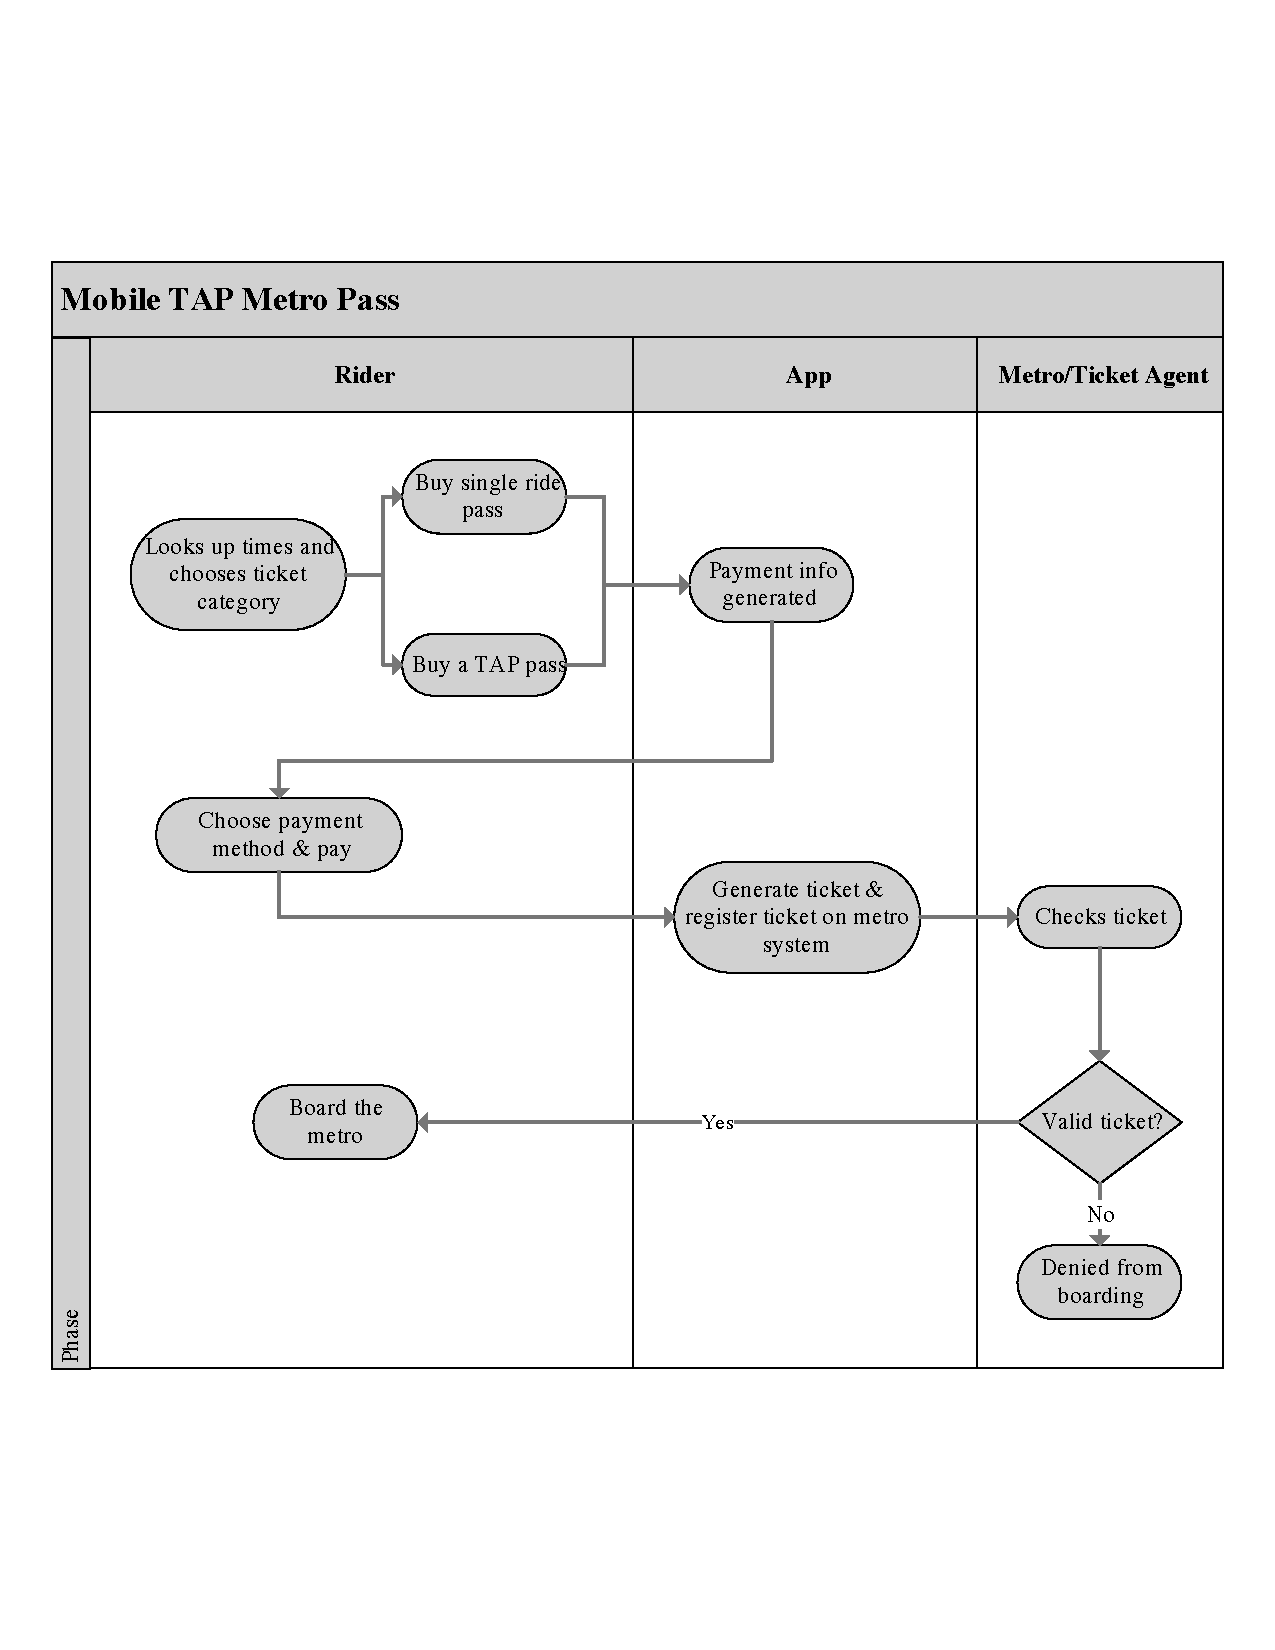
\includegraphics[scale=.355]{OCD/uml.pdf}
		\end{figure}